\documentclass[border=6pt]{standalone}
\usepackage{tikz}
\usetikzlibrary{arrows.meta,positioning,calc,shapes.geometric}
\begin{document}
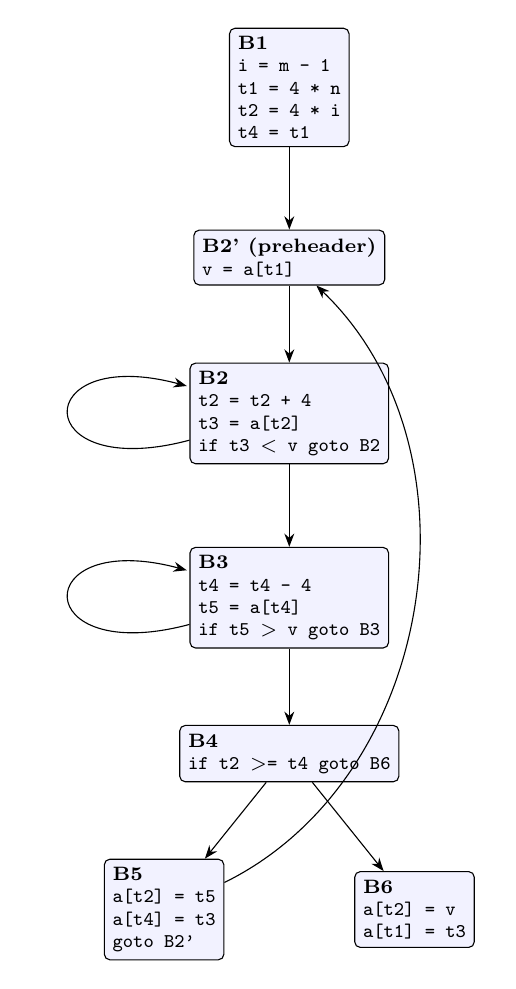
\begin{tikzpicture}[>=Stealth,font=\scriptsize,x=1.000cm,y=1.000cm,
 box/.style={draw,rounded corners=2pt,align=left,inner sep=3pt,fill=blue!5},
 circ/.style={draw,circle,align=center,inner sep=1pt,minimum size=0.75cm,fill=blue!5},
 lab/.style={font=\scriptsize,inner sep=1pt,fill=white,fill opacity=0.85,text opacity=1}]
\node[box] (b1) at (0.000,0.000) {\textbf{B1}\\\texttt{i = m - 1}\\\texttt{t1 = 4 * n}\\\texttt{t2 = 4 * i}\\\texttt{t4 = t1}};
\node[box] (b2p) at (0.000,-2.160) {\textbf{B2' (preheader)}\\\texttt{v = a[t1]}};
\node[box] (b2) at (0.000,-4.140) {\textbf{B2}\\\texttt{t2 = t2 + 4}\\\texttt{t3 = a[t2]}\\\texttt{if t3 \textless{} v goto B2}};
\node[box] (b3) at (0.000,-6.480) {\textbf{B3}\\\texttt{t4 = t4 - 4}\\\texttt{t5 = a[t4]}\\\texttt{if t5 \textgreater{} v goto B3}};
\node[box] (b4) at (0.000,-8.460) {\textbf{B4}\\\texttt{if t2 \textgreater{}= t4 goto B6}};
\node[box] (b5) at (-1.590,-10.440) {\textbf{B5}\\\texttt{a[t2] = t5}\\\texttt{a[t4] = t3}\\\texttt{goto B2'}};
\node[box] (b6) at (1.590,-10.440) {\textbf{B6}\\\texttt{a[t2] = v}\\\texttt{a[t1] = t3}};
\draw[->] (b1) --  (b2p);
\draw[->] (b2p) --  (b2);
\path[->] (b2) edge[loop left]  (b2);
\draw[->] (b2) --  (b3);
\path[->] (b3) edge[loop left]  (b3);
\draw[->] (b3) --  (b4);
\draw[->] (b4) --  (b5);
\draw[->] (b4) --  (b6);
\draw[->] (b5) to[bend right=55]  (b2p);
\end{tikzpicture}
\end{document}
